\documentclass{beamer}
\usepackage[galician]{babel}
\usepackage[utf8x]{inputenc}
\usepackage{fontenc}
\mode<presentation>{\usetheme[secheader]{Boadilla}}

\title{Obradoiro de introdución a Arduino}
\author[Brais, Rafa, Tucho]{ Brais \\ Rafa \\ Tucho}
\date{2014-10-08}

\begin{document}

\begin{frame}
\titlepage

licencia
logo bricolabs
logo gpul
\end{frame}

%% Indice de contidos
\begin{frame}{Indice}
  \tableofcontents
\end{frame}


\section{Hardware Libre}
\begin{frame}
\huge{\centerline{\textbf{\color{blue} \insertsection}}}
\end{frame}

\begin{frame}{Que é?}

\end{frame}

\begin{frame}{Proxectos}

\end{frame}



\section{Arduino}
\begin{frame}
\huge{\centerline{\textbf{\color{blue} \insertsection}}}
\end{frame}

\begin{frame}{Que é Arduino?}
% \frametitle{}
% \includegraphics[width=200pt]{./img/secam.png}
\begin{itemize}
 \item Controladoras
 \item IDE
 \item Comunidade
\end{itemize}

coller algo de http://arduino.cc/en/Guide/Introduction
\end{frame}

\begin{frame}{Arquitectura}
\begin{columns}[t]
	\begin{column}[t]{0.4\textwidth}
		\begin{itemize}
			\item micro
			\item reloxo
			\item controlador USB (todo)
			\item entradas saidas
			\item EEPROM
		\end{itemize}
	\end{column}
	\begin{column}[t]{0.6\textwidth}
		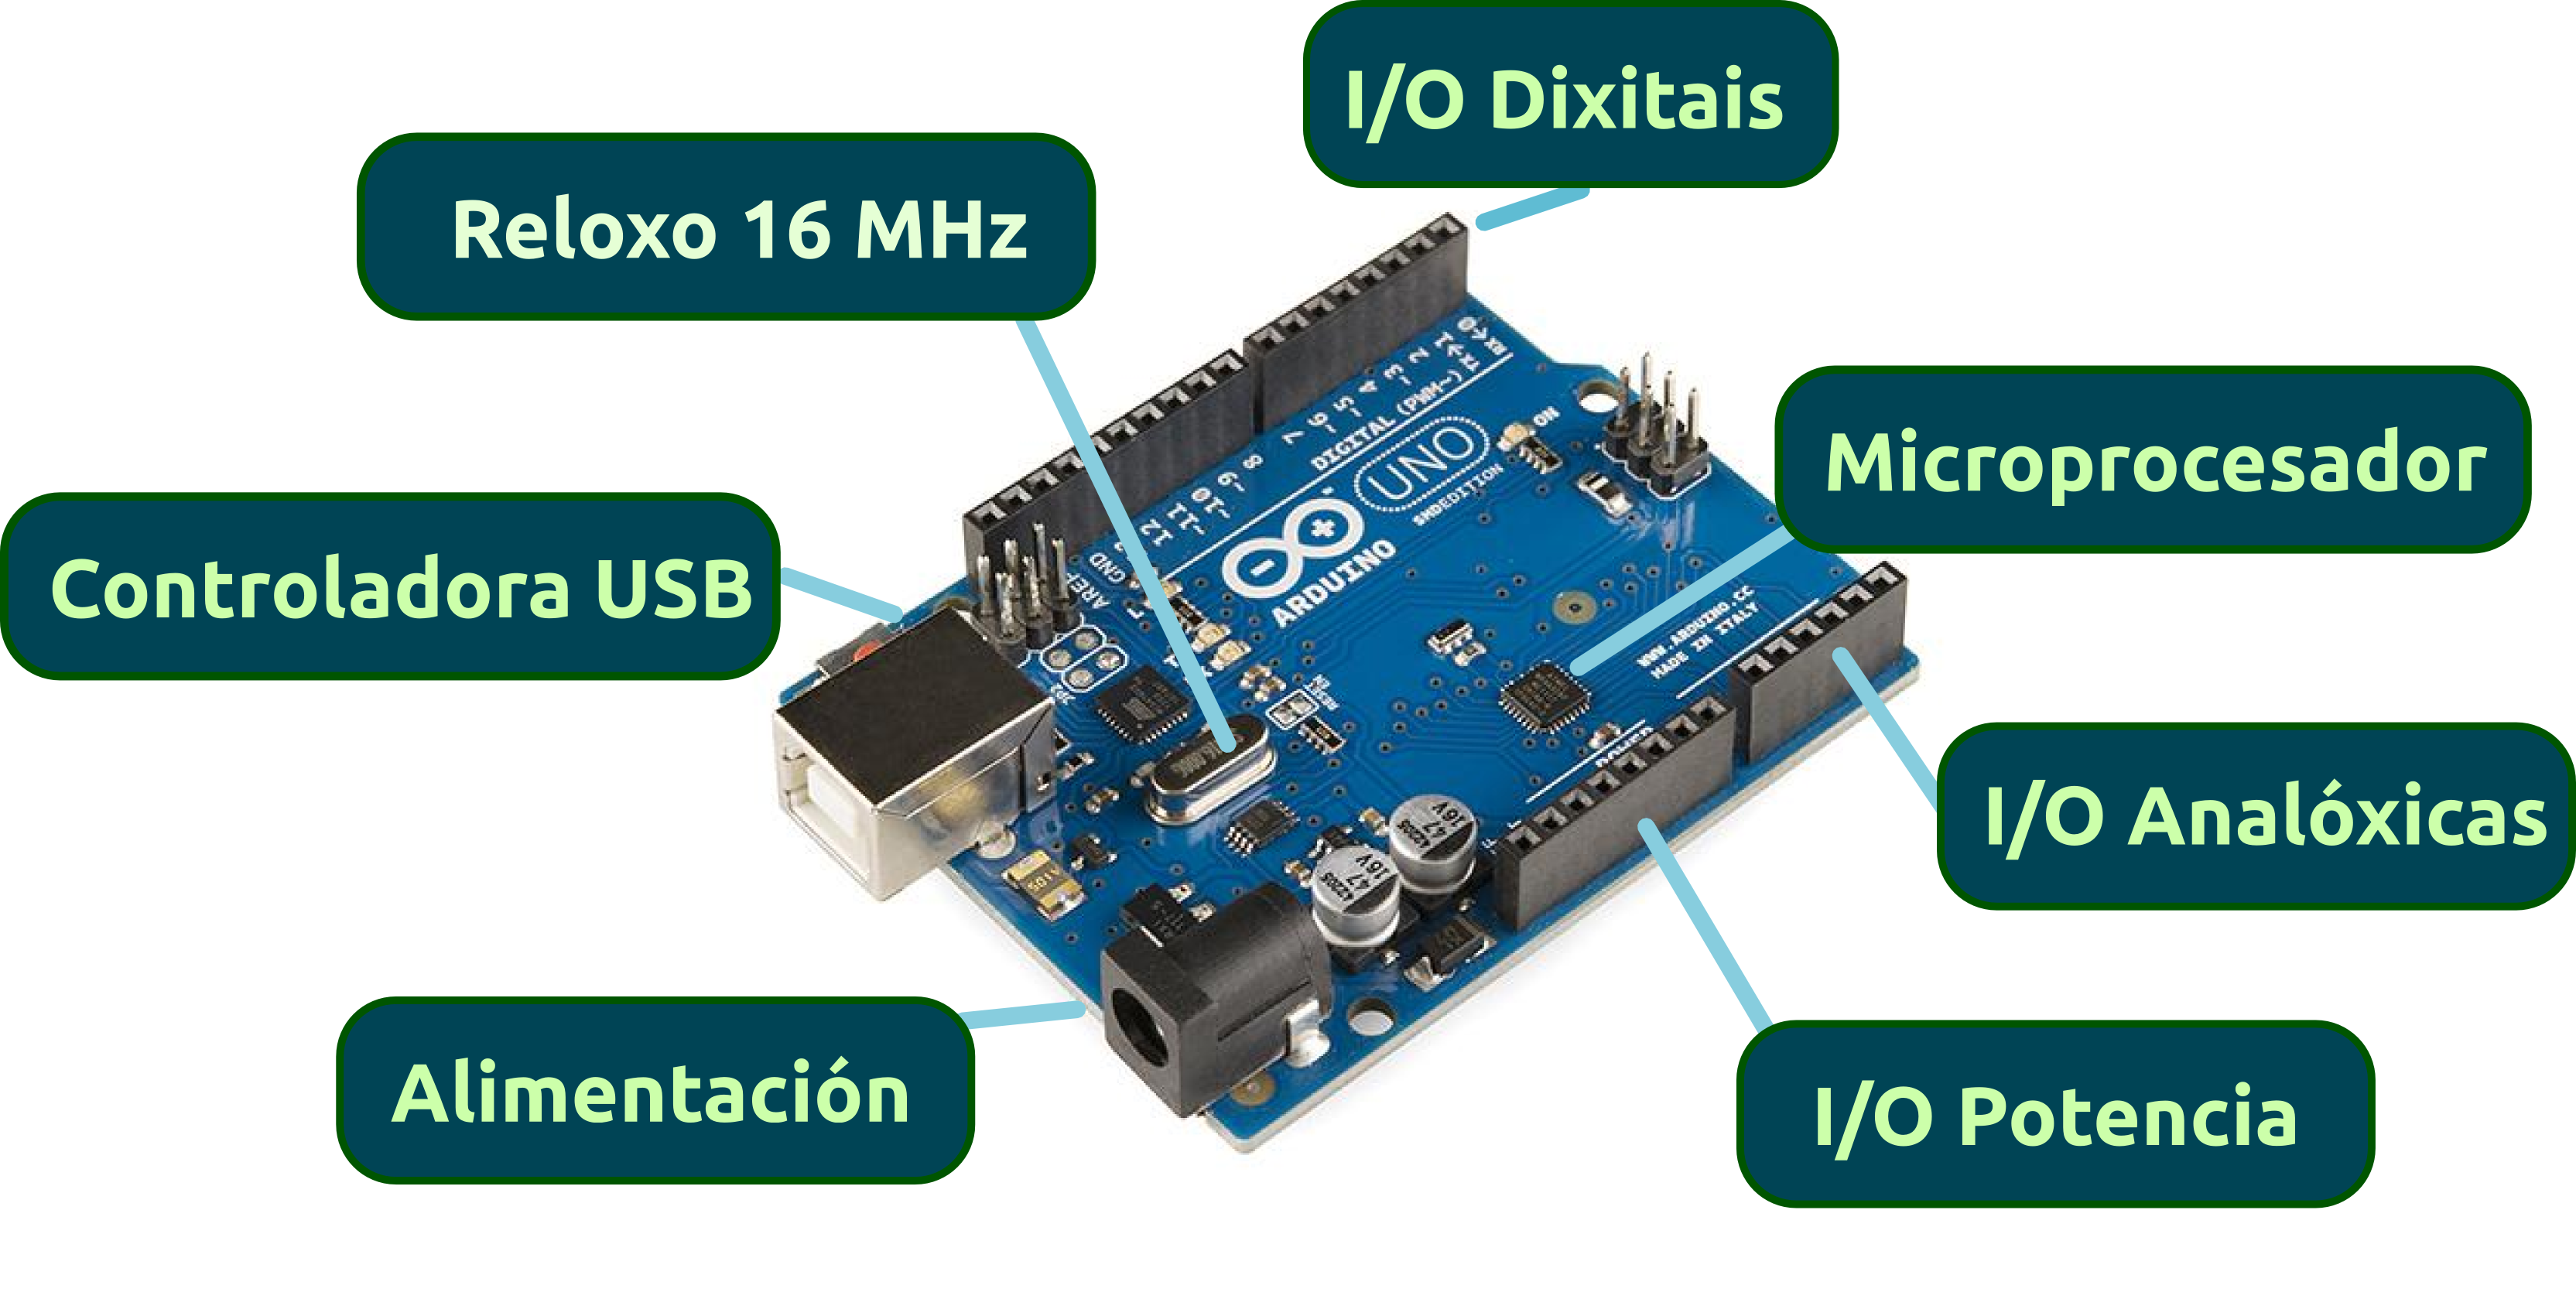
\includegraphics[width=200pt]{./img/arduinoUNOExplicado.png}
	\end{column}
\end{columns}
\end{frame}

\begin{frame}{Variedades}
COLUMNAS!
\begin{itemize}
 \item Placas
 \begin{itemize}
  \item UNO
  \item Mega
  \item Pro
  \item Micro
  \item Fio
  \item Robot
  \item LilyPad
 \end{itemize}

 \item Shields
\end{itemize}
% \includegraphics[width=200pt]{./img/secam.png}
\end{frame}

\begin{frame}{Onde buscar?}
\begin{itemize}
	\item http://arduino.cc
	\item http://arduino.cc/en/Tutorial/HomePage

\end{itemize}

\end{frame}


\section{A cacharrear!}
\begin{frame}
\huge{\centerline{\textbf{\color{blue} \insertsection}}}
\end{frame}

\begin{frame}{Blink}

\end{frame}


\begin{frame}{PWM e Blink}

\end{frame}


\begin{frame}{Temperatura}

\end{frame}

\begin{frame}{Sensor ultrasons}

\end{frame}

\begin{frame}{Imperial March}

\end{frame}
%
% %% Bibliografia
% \section{Bibliografía}
% \begin{frame}
%     \begin{thebibliography}{ZZ}
%
% 	\bibitem{torres}
% 	    Torres, Lleida, Casas Pla. \\
% 	    {\itshape Sistemas analógicos y digitales de televisión}. \\
% 	    Edicions UPC, 1993.
%
% 	\bibitem{Herve}
% 	    Benoi, Hervé. \\
% 	    {\itshape Digital television MPEG-1, MPEG-2 and principles of the DVB system}. \\
% 	    London: Arnold, 1997.
%
% 	\bibitem{wikipedia}
% 	    Varios Autores. \\
% 	    {\itshape Wikipedia}.
%     \end{thebibliography}
% \end{frame}
%
%
\end{document}
